\section*{WU4}
\begin{figure}[here]
	\center
	\caption{wu4}
	\label{fig:wu4}
	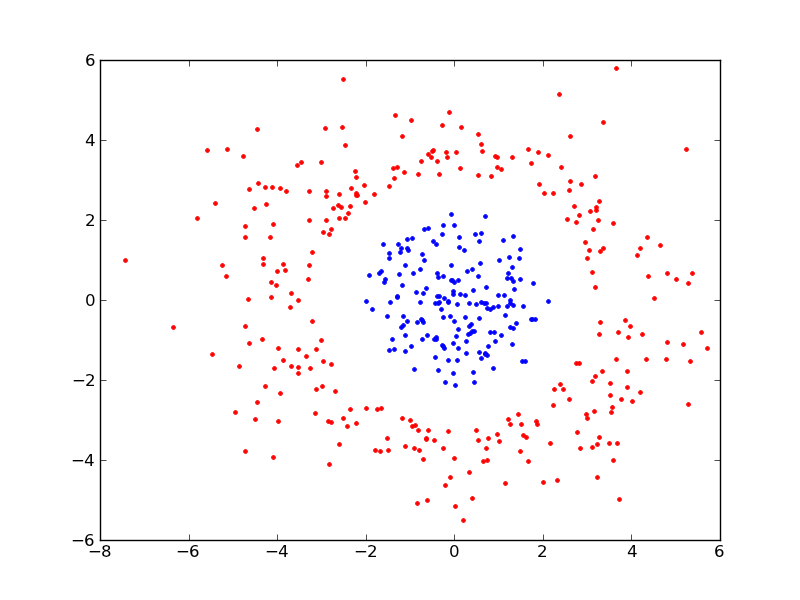
\includegraphics[width=4.0in]{img/wu4.png}
\end{figure}

Vanilla PCA will find this data difficult because variance of all directions are similar, 
which means that eigenvectors can point in any direction. 

Large eigenvalues means there is no correlation between any of the axis. 

\section*{WU5}
\begin{figure}[here]
	\center
	\caption{wu5}
	\label{fig:wu5}
	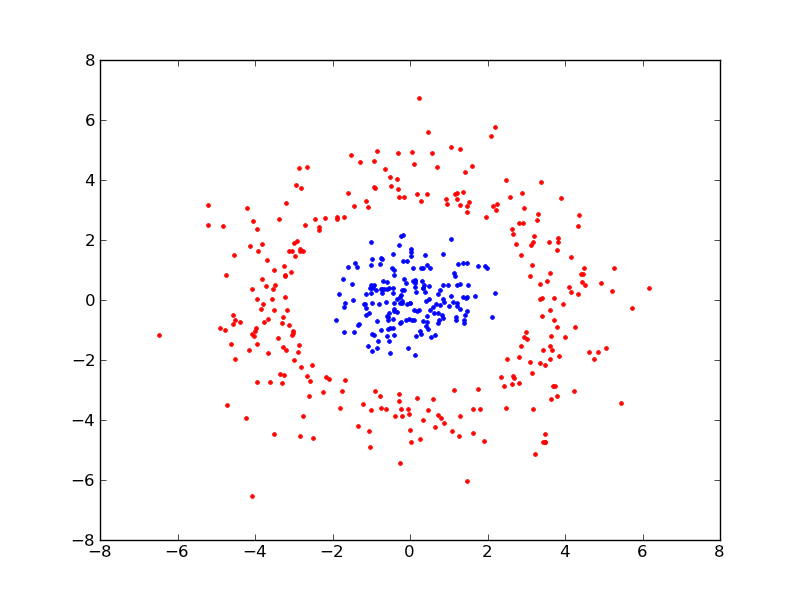
\includegraphics[width=4.0in]{img/wu5.png}
\end{figure}
PCA did not do what we want it to do :'(
In addition to the reasons listed in WU4, vanilla PCA 
did not do what we wanted to do because the data 
is not linearly separable.

\section*{WU6}
\begin{figure}[here]
	\center
	\caption{wu6}
	\label{fig:wu6}
	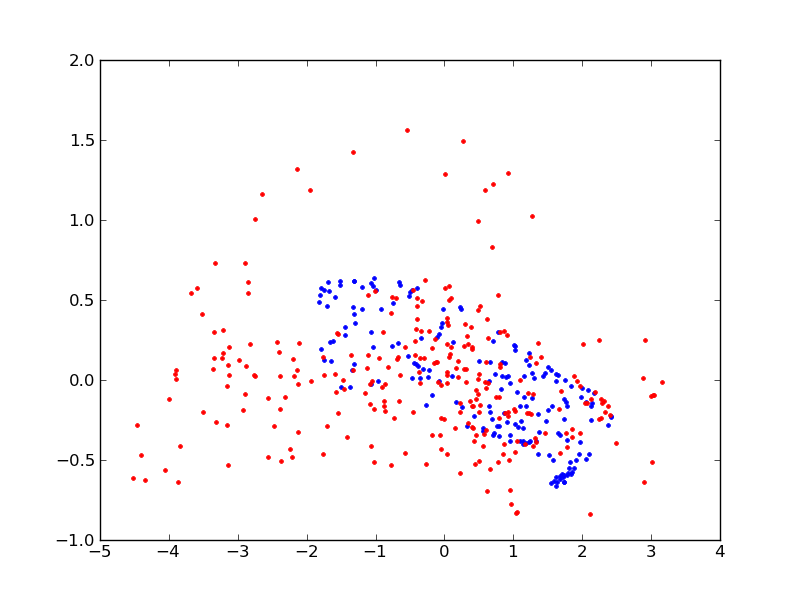
\includegraphics[width=4.0in]{img/wu6.png}
\end{figure}

Eignevalues here is [ 0.08228617  0.05882765], which is significantly smaller than
the eigenvalues for 
linear: [ 6.00010675  5.57361851]

\section*{WU7}
\begin{verbatim}
	linear: evals [ 6.00010675  5.57361851]
	poly2: [ 60.36960773  57.61047579]
	poly3: [ 2316.48011949  2139.88680252]
	rbf0_2: evals [ 0.15469386  0.10178237]
	rbf0_5: evals [ 0.1194342   0.06754455]
	rbf2: evals [ 0.05293176  0.04460633]
	rbf5: evals [ 0.02906865  0.02521906]
\end{verbatim}

\begin{figure}[here]
	\center
	\caption{wu7 linear}
	\label{fig:wu7_linear}
	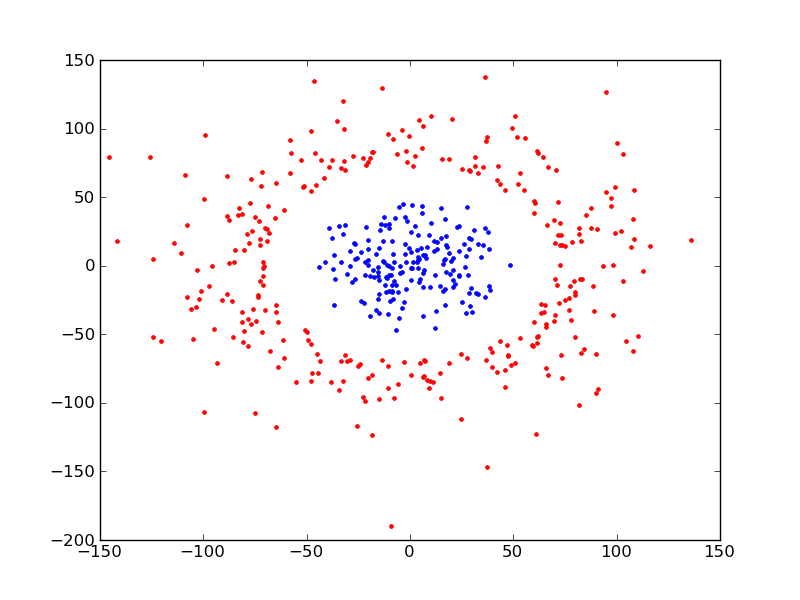
\includegraphics[width=4.0in]{img/wu7_linear.png}
\end{figure}

\begin{figure}[here]
	\center
	\caption{wu7 poly2}
	\label{fig:wu7_poly2}
	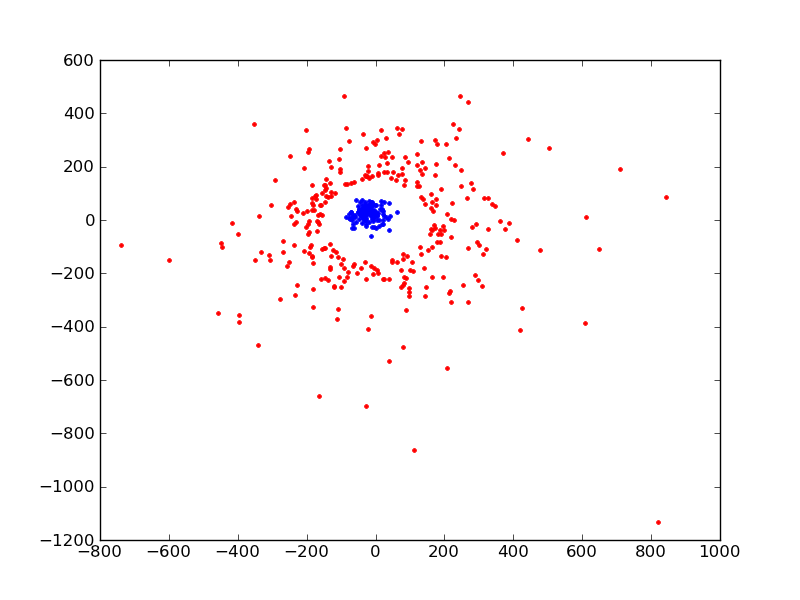
\includegraphics[width=4.0in]{img/wu7_poly2.png}
\end{figure}

\begin{figure}[here]
	\center
	\caption{wu7 poly3}
	\label{fig:wu7_poly3}
	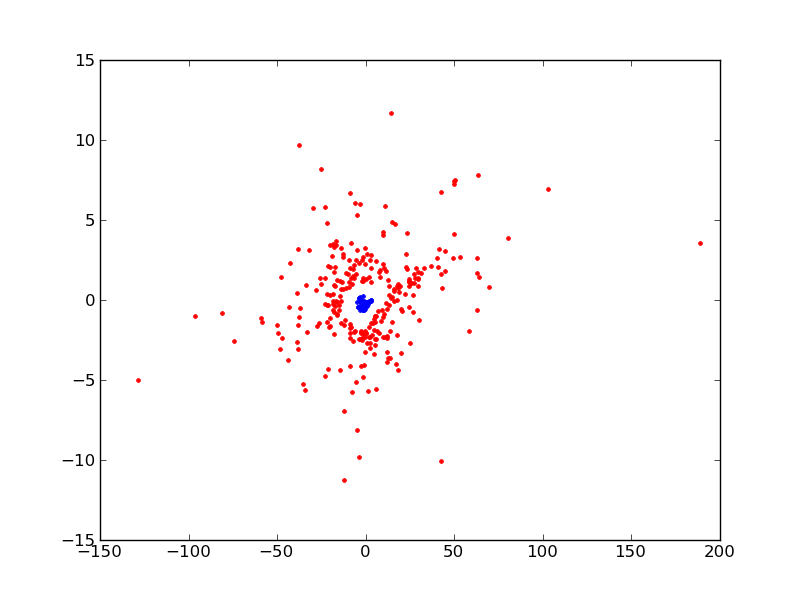
\includegraphics[width=4.0in]{img/wu7_poly3.png}
\end{figure}

\begin{figure}[here]
	\center
	\caption{wu7 rbf0.2}
	\label{fig:wu7_rbf0_2}
	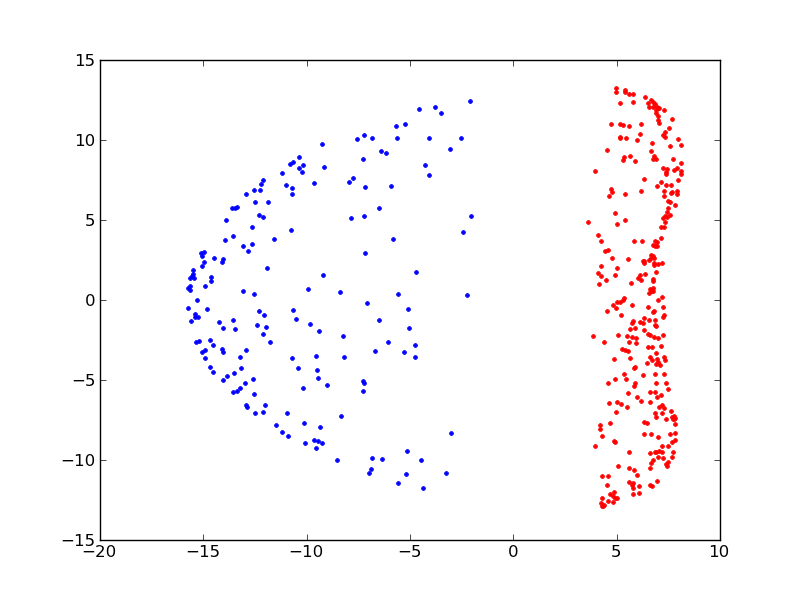
\includegraphics[width=4.0in]{img/wu7_rbf0_2.png}
\end{figure}

\begin{figure}[here]
	\center
	\caption{wu7 rbf0.5}
	\label{fig:wu7_rbf0_5}
	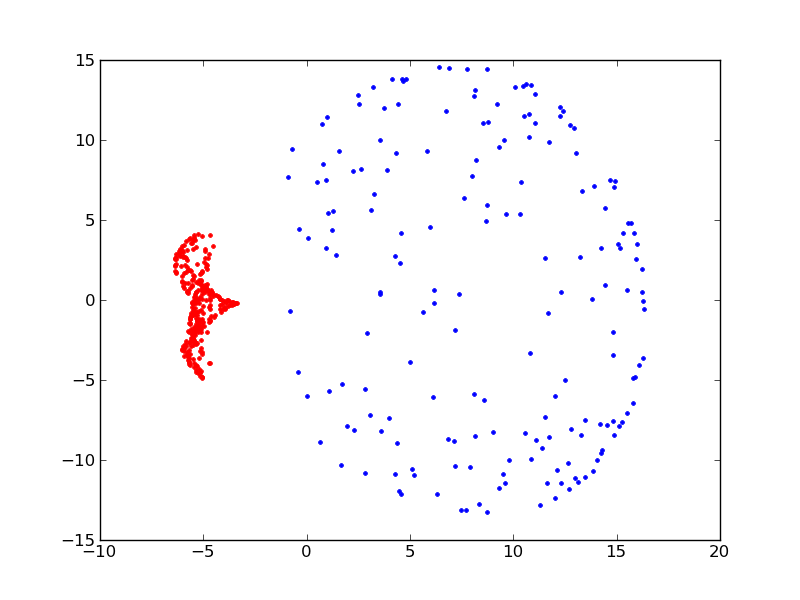
\includegraphics[width=4.0in]{img/wu7_rbf0_5.png}
\end{figure}

\begin{figure}[here]
	\center
	\caption{wu7 rbf1}
	\label{fig:wu7_rbf1}
	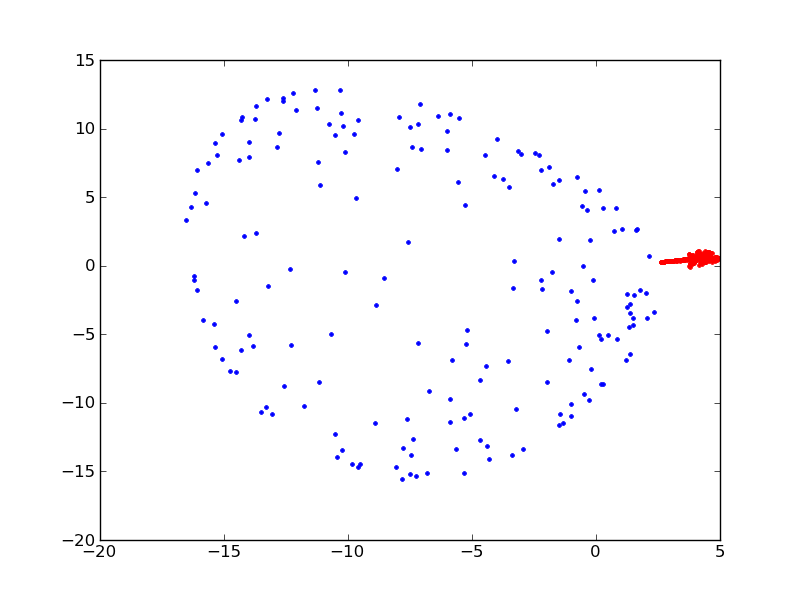
\includegraphics[width=4.0in]{img/wu7_rbf1.png}
\end{figure}

\begin{figure}[here]
	\center
	\caption{wu7 rbf2}
	\label{fig:wu7_rbf2}
	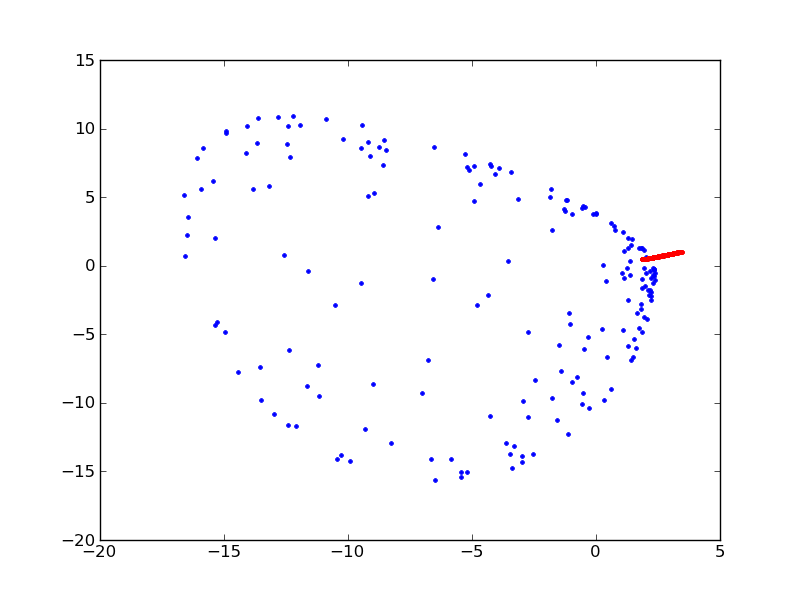
\includegraphics[width=4.0in]{img/wu7_rbf2.png}
\end{figure}

\begin{figure}[here]
	\center
	\caption{wu7 rbf5}
	\label{fig:wu7_rbf5}
	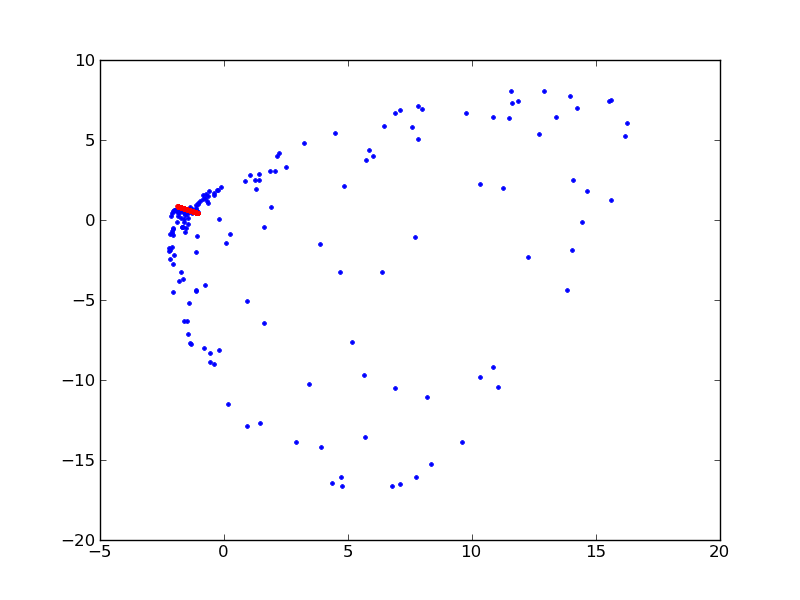
\includegraphics[width=4.0in]{img/wu7_rbf5.png}
\end{figure}